\chapter{Ход работы}

\section{Разработка Back-end}
Разработка back-end части велась на языке java с использованием технологии spring boot. В качестве системы сборки использовался maven, а версия java была выбрана 17.

Разработанный back-end возвращает данные о разработчиках сайта по технологии REST с использованием JSON в виде способа представления информации. Такой подход является наиболее популярным в настоящее время.

\section{Разработка Front-end}
Разработка front-end части велась с использованием html, css и js. Для построения приложения применялся framework React.

В ходе разработки использовались следующие теги для вставки медиа-контента на страницу:
\begin{itemize}
	\item <audio> --- для вставки аудио
	\item <iframe> --- для вставки видео с YouTube
	\item <img/> --- для вставки изображений из различных источников
\end{itemize}

Для обеспечения интеграции аудио с приложением был написан собственный плеер, который в первой итерации разработки может воспроизводить видео, ставить его на паузу, сбрасывать на начало, показывать общее и текущее вермя в секундах, а также отображать название аудиозаписи.

\section{Демонстрация работы}

\begin{figure}[H]
	\centering
	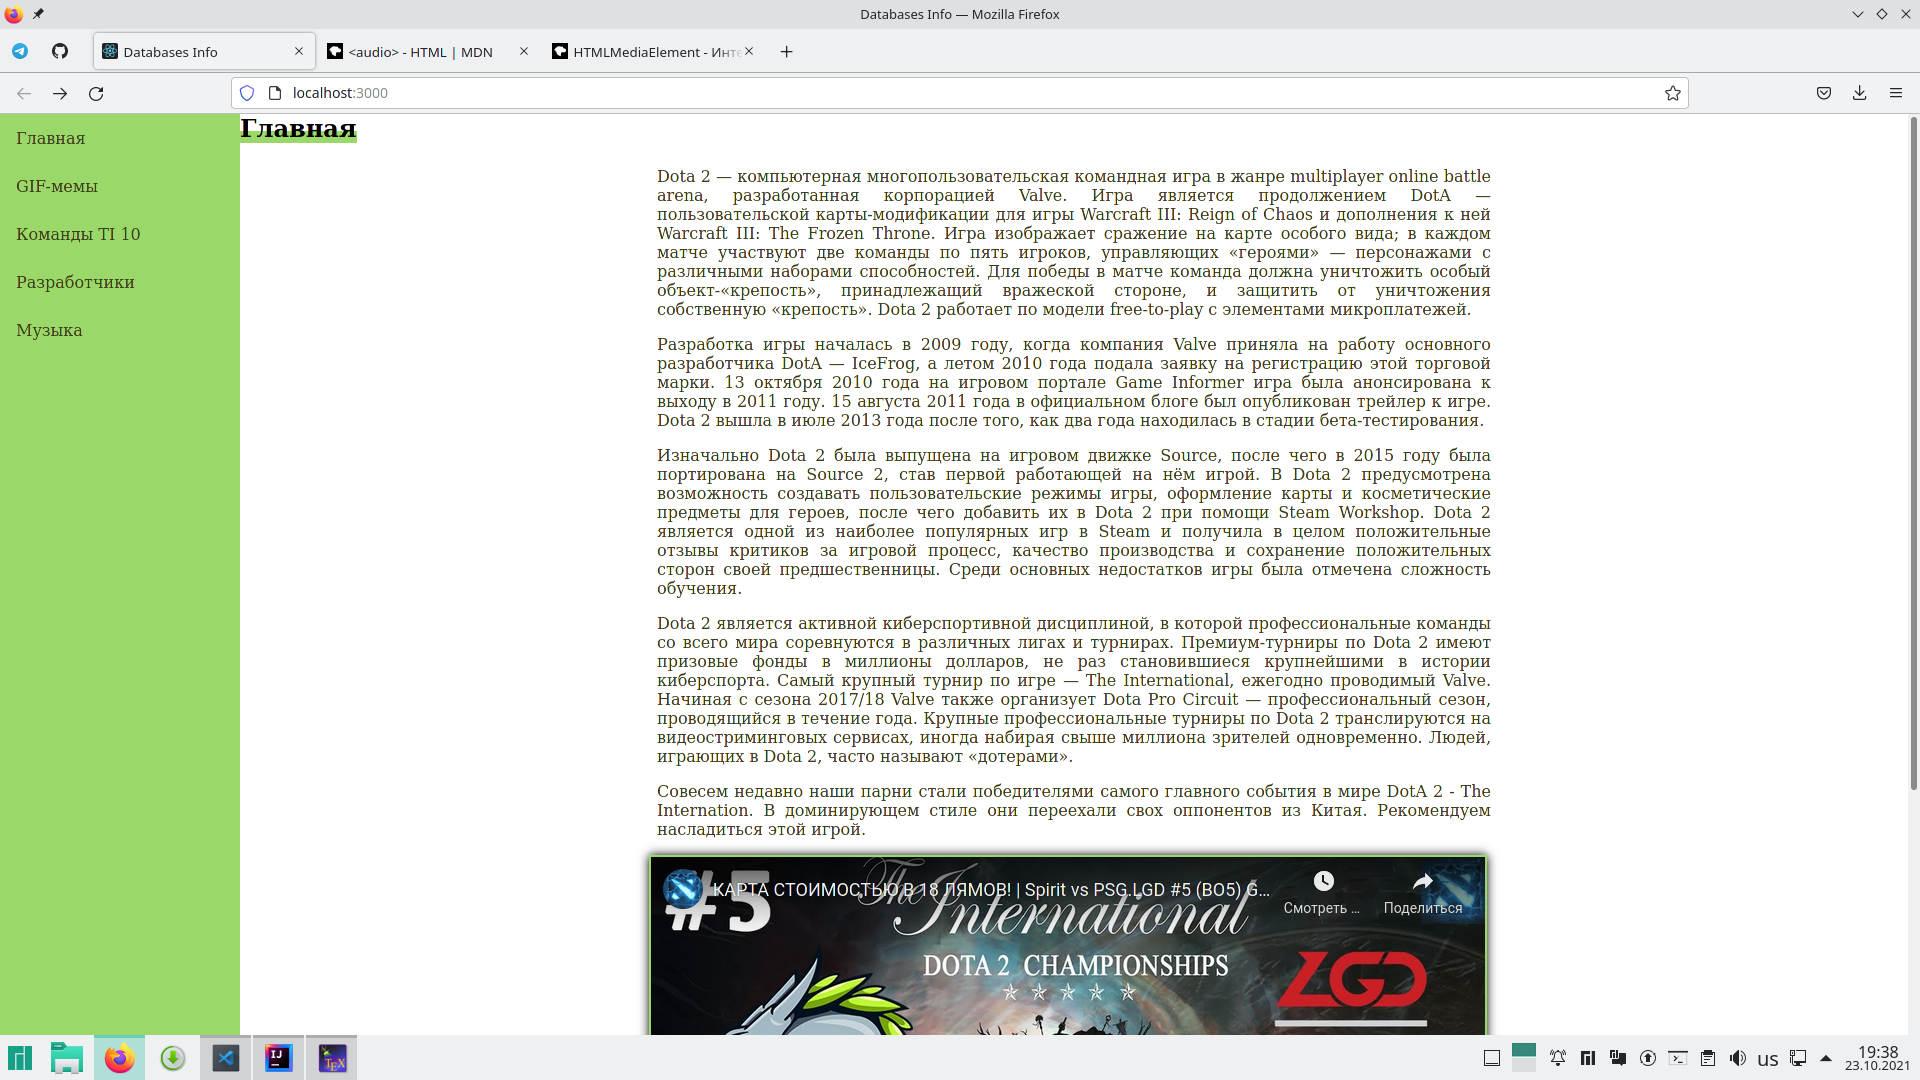
\includegraphics[width=\linewidth]{01}
	\caption{Главная страница}
\end{figure}

\begin{figure}[H]
	\centering
	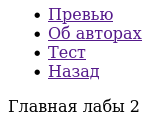
\includegraphics[width=\linewidth]{02}
	\caption{GIF'ки}
\end{figure}

\begin{figure}[H]
	\centering
	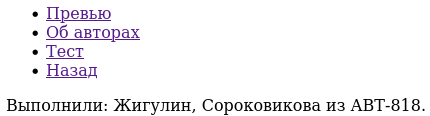
\includegraphics[width=\linewidth]{03}
	\caption{Команды TI10}
\end{figure}

\begin{figure}[H]
	\centering
	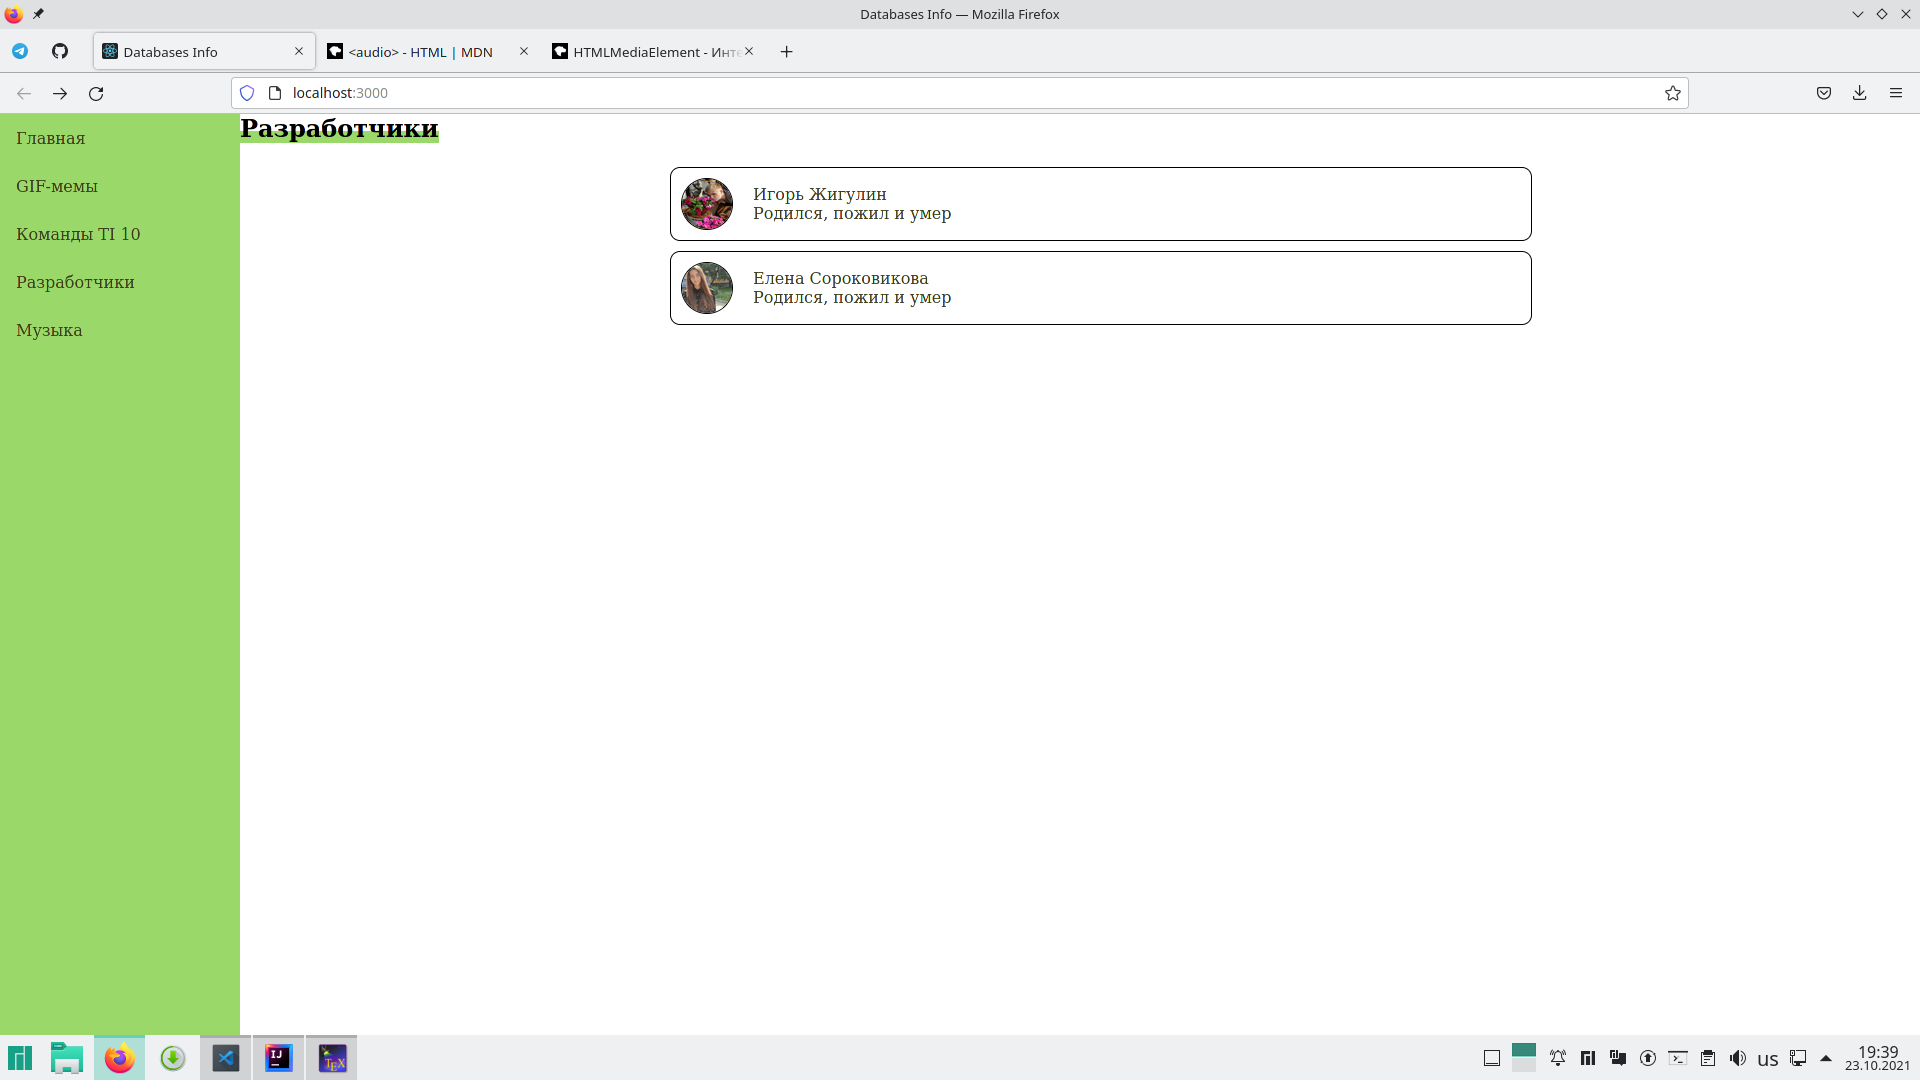
\includegraphics[width=\linewidth]{04}
	\caption{Разработчики}
\end{figure}

\begin{figure}[H]
	\centering
	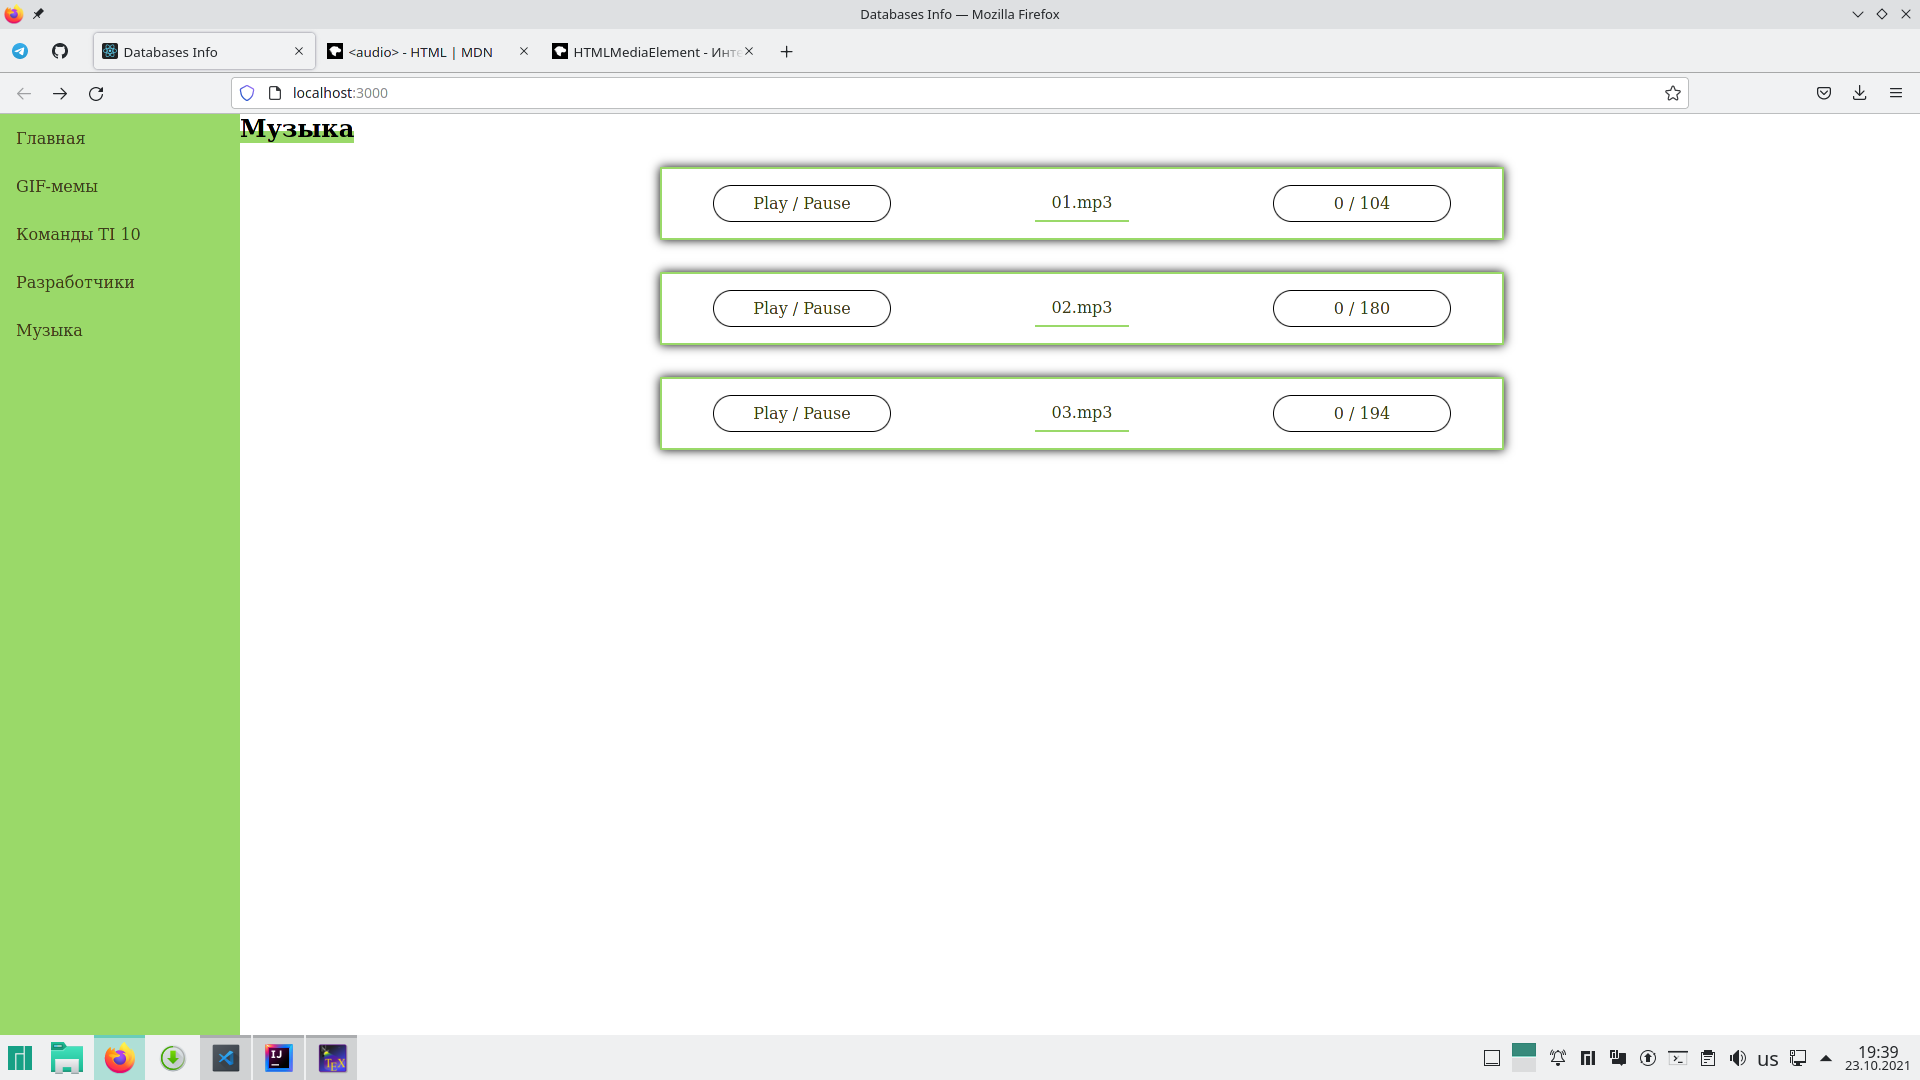
\includegraphics[width=\linewidth]{05}
	\caption{Музыка}
\end{figure}
